\section{Pyserial Mindwave}
NeuroSky Mindwave EEG adalah alat yang digunakan dalam penelitian ini dan alat terhubung ke Kode Python sebagai bahasa pemrograman yang digunakan sehingga menampilkan sinyal mentah nyata. Serta menggunakan pyserial merupakan modul Python siap-pakai dan gratis yang dibuat untuk memudahkan kita dalam membuat program komunikasi data serial RS232 dalam bahasa Python.

\section{Code Program Mindwave}
\subsection{Code Program Pyserial Function Pada Mindwave}
\begin{enumerate}
\item Berikut Codingan Function Untuk Menampilkan Gelombang Otak pada Mindwave seperti pada listing \ref{lst:gomw} : 
\lstinputlisting[caption=Function Untuk Menampilkan Gelombang Otak pada Mindwave, label={lst:gomw}]{src/4/gomw.py}
Pada listing \ref{lst:gomw}: menunjukkan adanya pemberian ukuran pada grafik gelombang otak, dan menampilkan  gelombang otak dalam grafik. Berikut gambar \ref{fig:gomw} hasil dari function menampilkan gelombang otak.
\begin{figure}[!htbp]
	\centerline{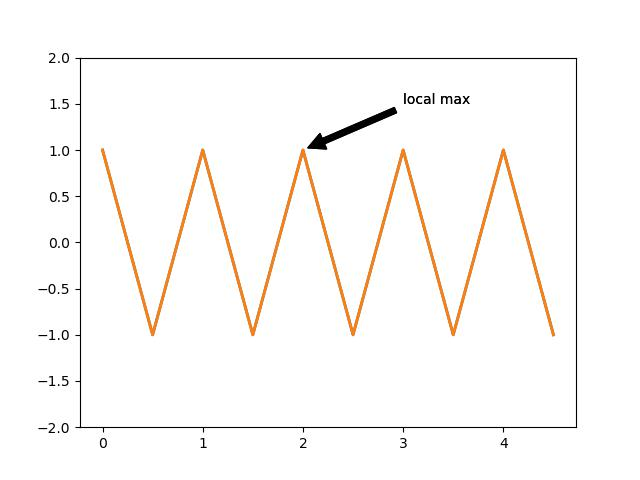
\includegraphics[width=0.85\textwidth]{figures/4/gomw.PNG}}
	\caption{function menampilkan gelombang otak}
	\label{fig:gomw}
\end{figure}

\item Codingan Function Memasukan Data Plotting Pada Mindwave seperti pada listing \ref{lst:dpmw} : 
\lstinputlisting[caption=Function Memasukan Data Plotting Otak pada Mindwave, label={lst:dpmw}]{src/4/dpmw.py}
Pada listing \ref{lst:dpmw} menunjukan bahwa adanya penambahan pada data plotting dengan memberikan judul pada grafik gelombang otak serta memberikan keterangan waktu dan voltage. Berikut hasil dari codingan pada function memasukkan data plotting seperti pada gambar \ref{fig:dpmw} :
\begin{figure}[!htbp]
	\centerline{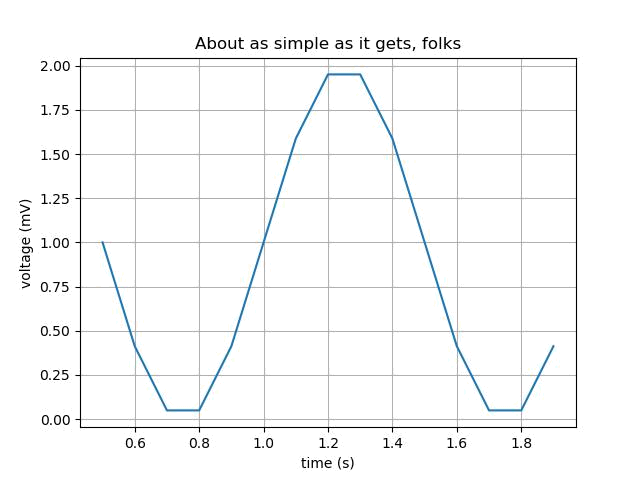
\includegraphics[width=0.85\textwidth]{figures/4/dpmw.PNG}}
	\caption{function Data Plotting pada Mindwave}
	\label{fig:dpmw}
\end{figure}

\item Code Program Function Sub.plot Pada Mindwave seperti pada listing \ref{lst:spmw} : 
\lstinputlisting[caption=Function Subplot pada Mindwave, label={lst:spmw}]{src/4/spmw.py}
Pada listing \ref{lst:spmw} menjelaskan bahwa adanya perubahan pada sub.plot mindwave ini yang menunjukkan tampilan grafik gelombang otak dengan ukuran gambar yang kecil. Berikut hasil dari codingannya seperti pada gambar \ref{fig:spmw} :
\begin{figure}[!htbp]
	\centerline{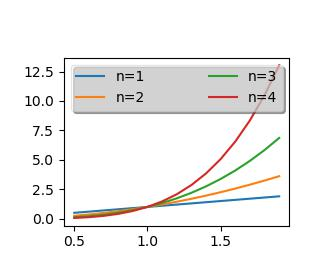
\includegraphics[width=0.85\textwidth]{figures/4/spmw.PNG}}
	\caption{function Subplot pada Mindwave}
	\label{fig:spmw}
\end{figure}

\item Code Program Function Memberikan Keterangan Waktu dan Frekuensi seperti pada listing \ref{lst:kwf} : 
\lstinputlisting[caption=Function Memberikan Keterangan Waktu dan Frekuensi, label={lst:kwf}]{src/4/kwf.py}
Pada listing \ref{lst:kwf} mejelaskan adanya penambahan function keterangan waktu dan frekuensi pada pyserial mindwave.
Berikut hasil dari codingannya seperti pada gambar \ref{fig:kwf} :
\begin{figure}[!htbp]
	\centerline{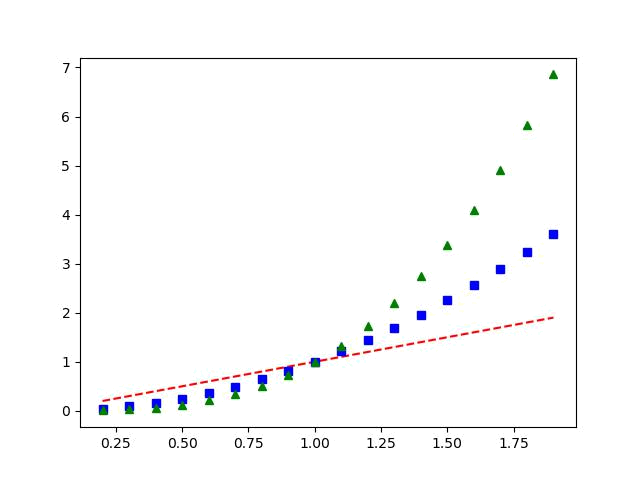
\includegraphics[width=0.85\textwidth]{figures/4/kwf.PNG}}
	\caption{Function Memberikan Keterangan Waktu dan Frekuensi}
	\label{fig:kwf}
\end{figure}

\item Code Program Function Memasukkan Rumus Pada Grafik Gelombang Otak seperti pada listing \ref{lst:rumusgrafik} : 
\lstinputlisting[caption=Function Memasukkan Rumus Pada Grafik Gelombang Otak, label={lst:rumusgrafik}]{src/4/rumusgrafik.py}
Pada listing \ref{lst:rumusgrafik} mejelaskan adanya penambahan function memasukkan rumus gelombang otak pada pyserial mindwave.
Berikut hasil dari codingannya seperti pada gambar \ref{fig:rumusgrafik} :
\begin{figure}[!htbp]
	\centerline{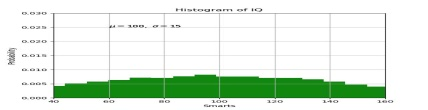
\includegraphics[width=0.85\textwidth]{figures/4/rumusgrafik.PNG}}
	\caption{Function Memasukkan Rumus Pada Grafik Gelombang Otak}
	\label{fig:rumusgrafik}
\end{figure}
\end{enumerate}

\section{Tutorial Mengatasi error Pyserial Function pada Mindwave}
\subsection{Mengenal error Dalam Program}
Pada bahasa pemrograman, terdapat bahasa yang berbasis dekstop,web,dan lain-lain. Misalnya di dalam bahasa C, setiap pernyataan harus diakhiri dengan titik koma, namun pada visual basic tidak perlu digunakan.

Saat kita menjalankan suatu program dalam  bahasa pemrograman menemukan kesalahan pada sintaks atau codingan di dalam suatu prorgam sehingga menyebabkan program tidak berjalan dengan baik.

Dilihat dari jenis kesulitan dalam memperbaiki suatu program, terdapat 3 kesalahan yaitu :
\begin{enumerate}
\item error Tata Bahasa (Sintaks)

Merupakan jenis error yang sering terjadi dalam pembuatan program. Namun error ini sangat mudah terdekteksi karena umumnya compier dari masing-masing bahasa program sebelum program  di jalankan.

\item Error Runtime

Merupakan tingkatan dimana error ini dapat terdeksi saat program dijalakan. Penyebabnya beragam, karena terjadinya kesalahan dalam proses input,serta perhitungan saat proses output.

\item Error Logika (Logical Error)

Merupakan jenis error yang sangat sulit terdeteksi karena terjadinya bukan karena kesalahan pada penulisan sintaks,melainkan dari kesalahan programmer dalam menggunakan algoritma.
\end{enumerate}

\subsection{Code error Pada Program Pyserial Mindwave}
\begin{enumerate}
\item Error no attribute
Hasilnya seperti pada gambar \ref{fig:errorna} :
\begin{figure}[!htbp]
	\centerline{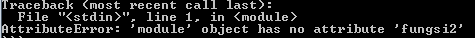
\includegraphics[width=0.85\textwidth]{figures/4/errorna.PNG}}
	\caption{Error no attribute}
	\label{fig:errorna}
\end{figure}
Jika Masih ada yang error di kodingnya. Perhatikan lagi kodingnya.

\item Error Indentation
Hasilnya seperti pada gambar \ref{fig:errori} :
\begin{figure}[!htbp]
	\centerline{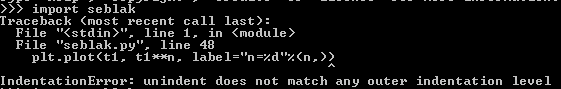
\includegraphics[width=0.85\textwidth]{figures/4/errori.PNG}}
	\caption{Error Indetation}
	\label{fig:errori}
\end{figure}
Berarti masih ada yang error dalam jarak spasi coba di sesuaikan dengan baris
Yang lain.

\item Error Parameter
Hasilnya seperti pada gambar \ref{fig:errorp1} :
\begin{figure}[!htbp]
	\centerline{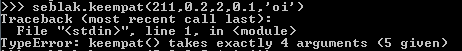
\includegraphics[width=0.85\textwidth]{figures/4/errorp1.PNG}}
	\caption{Error Parameter}
	\label{fig:errorp1}
\end{figure}
Jika terjadi error seperti di atas berarti kita memasukkan parameternya
Kelebihan  atau kekurangan. Jadi sesuaikan parameter yang anda isi dengan
Kodingan.

\item Error parameter 
Hasilnya seperti pada gambar \ref{fig:errorp2} :
\begin{figure}[!htbp]
	\centerline{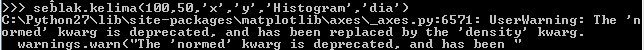
\includegraphics[width=0.85\textwidth]{figures/4/errorp2.PNG}}
	\caption{Error Parameter}
	\label{fig:errorp2}
\end{figure}
Jika terjadi seperti diatas maka cek dulu nama parameternya, kemungkinan masih terjadi   kesalahan penulisan.

\item Error Penulisan
Hasilnya seperti pada gambar \ref{fig:errorpn} :
\begin{figure}[!htbp]
	\centerline{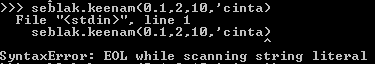
\includegraphics[width=0.85\textwidth]{figures/4/errorpn.PNG}}
	\caption{Error Penulisan}
	\label{fig:errorpn}
\end{figure}
Jika terjadi error seperti diatas, maka perhatikan penggunan tanda baca.
\end{enumerate}